\chapter{Metodologías}
En todo proyecto es necesaria una metodología que ayude a guiar el siguiente paso, ya que en realidad el paso más importante es el siguiente y no el primero. Por esta razón, en este capítulo se describirá la metodología utilizada así como la planificación del proyecto.

\section{Marco ágil del proyecto}
Debido a las limitaciones de la gestión de proyectos, a finales de los 90 se empezó a utilizar una metodología ágil. Pero no fue hasta 2001 que un grupo de expertos desarrolla el ``Manifiesto por el Desarrollo Ágil de Software''. Donde se especificaron los doce principios clave para el desarrollo de software. A partir de ese punto, cada vez han ido surgiendo más modelos ágiles. Los 12 conceptos clave\cite{OBS2016} a seguir en este proyecto son\:
\begin{enumerate}
    \item Los cambios son bienvenidos
    \item Software funcional en un periodo corto de tiempo
    \item Facilidad para medir el progreso
    \item Desarrollo sostenible
    \item Excelencia técnica y buen diseño
    \item Simplicidad
    \item Adaptación a circunstancias cambiantes
\end{enumerate}

\section{Design Thinking}
En el proyecto, se aplicará el enfoque del \gls{design thinking}, en el que sus primeros pasos implican realizar un análisis del problema empatizando con los usuarios y para la definición del usuario se utilizará la metodología de personas. Para empatizar con el usuario y comprender a fondo el problema que están experimentando, se debe asumir el rol de usuario y ponerse en su lugar para identificar los posibles obstáculos que podrían tener al cocinar con ingredientes específicos sin conocer una receta adecuada. En este caso, el proceso de \gls{design thinking} nos ayudará a resolver el problema del usuario al permitirle encontrar recetas que se adapten a los ingredientes de su elección, abordando así sus necesidades de manera efectiva.

El concepto nació a finales del siglo XX como un compuesto que se basa en disciplinas como el diseño industrial y gráfico, además de la ingeniería y arquitectura. Este se refiere a estrategias creativas que utilizan los diseñadores durante el proceso de diseño. También es utilizado tanto como para abordar problemas como para desarrollar una solución, no solo en el ámbito de la ingeniería sino en ámbitos como empresas o cuestiones sociales. El \gls{design thinking} aprovecha los métodos a disposición del diseñador para hacer coincidir las necesidades de las personas con lo tecnológicamente factible, que a su vez se puede convertir en valor de mercado para una empresa.

Se compone de cinco estados que se deben usar en el proceso. Es muy importante no saltarse ningún paso
\begin{figure}[h]
    \begin{enumerate}
        \item Empatizar
        \item Definir
        \item Idear
        \item Crear prototipos
        \item Pruebas
    \end{enumerate}
    \caption{Pasos en el design thinking}
    \label{list:stepsDesign}
\end{figure}

Se determinan las características de los usuarios objetivo de los que se van a beneficiar de la aplicación. Así es posible obtener toda la información posible sobre los usuarios del producto y sus necesidades. Este paso ya se ha realizado anteriormente y se han especificado los clientes de la aplicación.

La siguiente etapa del \gls{design thinking} es la definición del usuario, es el paso más difícil ya que normalmente el desarrollador del proyecto tiende a idear soluciones familiares para él, pero se tiene que poner al usuario por delante de la comodidad del desarrollador. Se perfilarán los usuarios del proyecto, detallando su entorno, conocimientos, círculos sociales, motivaciones, etc... Para comprender que necesidades tienen de la aplicación. Basándonos en esas necesidades irán surgiendo nuevos objetivos y metas que alcanzar.

El paso de idear involucra la parte creativa del diseño, se debe intentar generar la mayor cantidad de ideas posibles, teniendo en cuenta solo las más importantes o realistas en el proyecto. Y una vez que se ha realizado una lluvia de ideas se seleccionarán las más relevantes y se creará un prototipo de aplicación, o varios dependiendo del proyecto. Para la fase de pruebas, donde se debería llegar al mayor público posible para obtener la mayor cantidad de retroalimentación de cara a futuras versiones de la aplicación o el descubrimiento de nuevas necesidades del usuario. \cite{wolniak2017design}

Para realizar los pasos futuros del \gls{design thinking} se tendrá en cuenta lo explicado en este apartado, en la etapa de ideas se anotarán las ideas más relevantes para la solución al problema de los usuarios. Posteriormente se escogerán las ideas más relevantes y razonables para crear prototipos de la aplicación planteada en el proyecto. Y, por último, se presentará el prototipo a determinados usuarios que puedan aportar retroalimentación útil para posibles mejoras o nuevas necesidades que se deban cubrir.

\subsection{Empatizar - User journeys}

En primer lugar se tratará de resolver el problema de un estudiante que cuenta con un presupuesto ajustado al mes y no puede permitirse el lujo de comprar en el supermercado todos los días. Dicho estudiante se siente frustrado por no ser capaz de controlar sus gastos en el supermercado y que ciertos ingredientes que no utiliza asiduamente le caduquen en la despensa. Por casualidad descubre el software desarrollado en este proyecto y se lo descarga. Una vez descargado abre la aplicación e introduce los ingredientes que tiene en su despensa. El estudiante podrá encontrar a su disposición diferentes recetas que realizar con los ingredientes introducidos. Una vez seleccionada la receta, el usuario puede comprobar los detalles de la misma.

Otro problema que se tratará de resolver es el que tiene una persona mayor que no se encuentra en disposición de ir al supermercado cada vez que le faltan ingredientes y tiene una despensa limitada. De pronto escucha la existencia de la aplicación y se dispone a probarla. Después de descargarla, con dificultad debido a sus achaques de la edad y a su dificultad para entender las nuevas tecnologías, la abre. En primer lugar debe introducir los ingredientes que tiene por casa y aunque encuentra cierta dificultad sustituir una nota de papel, con esfuerzo consigue hacer un inventario de sus ingredientes. La aplicación en este momento le podrá empezar a sugerir recetas con los ingredientes que tiene en su despensa. Después de elegir una receta, puede comprobar los detalles de la misma con detenimiento.

\subsection{Definir - Perfiles de usuarios}
Para definir a los usuarios se utiliza la metodología de personas. 

El concepto surge del intento de comprender coherentemente fue muy utilizado en los 90. Antiguamente en marketing para definir audiencias se utilizaba un método menos preciso. Se pensaba en personas que pudiesen ser un \emph{target} para el producto, teniendo en cuenta pocas características. En un ejemplo de productos de bebé, se consideraba la edad de los padres, la del bebé y opcionalmente el poder adquisitivo. Con la metodología de persona es posible profundizar mucho más a la hora de de identificar audiencias.\cite{persona2019}

Para construir personas se detallan una serie de preguntas que permiten perfilar el cliente del producto. Se responderán las siguientes preguntas:
\begin{enumerate}
    \item ¿Cómo se llama?
    \item ¿Qué edad tiene?
    \item ¿A que se dedica?
    \item ¿Qué idiomas domina?
    \item ¿Cómo es la persona?
    \item ¿Qué dispositivos tiene?
    \item ¿Cuál es su entorno social?
    \item ¿Qué le motiva?
    \item ¿Cuál es la frase que le inspira?
\end

\subsubsection{Perfil de un estudiante}
\begin{itemize}
    \item Nombre: Daniel Pérez
    \item Edad: 22 años
    \item Ocupación: Estudiante de Bioquímica
    \item Idiomas: Español, inglés y francés
    \item Descripción general: Daniel cursa el tercer año de su carrera en Bioquímica en una universidad pública, ansioso por frenar el hambre en el mundo, investigando una manera de crear cultivos que arraiguen en climas extremadamente secos. Divide su tiempo entre las clases, trabajos y amigos. Lee multitud de investigaciones científicas actuales, estando muy interesando en este mundo.
    \item Dispositivos: Daniel utiliza asiduamente el ordenador y vive enganchado al teléfono.
    \item Entorno social: Las amistades de Daniel son también estudiantes que están acabando sus estudios y se plantean iniciarse en el mundo laboral. Se dedican a diferentes campos no solo científicos. Pero todos están muy concienciados con las causas sociales. En el ámbito familiar, Daniel tiene una relación cercana con sus padres y su hermano Jorge. Realizan actividades habituales en familia y están todo el tiempo que pueden juntos. Aunque él viva en un piso para estudiantes con tres personas más.
    \item Motivación: Daniel busca reducir el derroche de alimentos que se ponen malos en su piso. Ya que en ocasiones se olvidan de algún ingrediente que se termina poniendo malo. Además, cuenta con unos recursos realmente limitados. 
    \item Cita: Erradicar el hambre en el mundo es una responsabilidad compartida.
\end{itemize}

\subsubsection{Perfil de una persona mayor}
\begin{itemize}
    \item Nombre: María Encarnación Sánchez
    \item Edad: 85 años
    \item Ocupación: Jubilada
    \item Idiomas: Español
    \item Descripción general: Maria Encarnación vive en un pequeño barrio al norte de Granada, donde las calles son demasiado empinadas para ir tirando del carrito de la compra por los inmensos escalones hasta el supermercado y vuelta. Muchos días piensa que ya no tiene edad para estar yendo a comprar cada dos o tres días, aunque no tenga mucho más que hacer. Se pasa las mañanas realizando tareas del hogar. Aunque cuando encuentra un hueco, se arregla para ir a su parroquia, ubicada a tan solo unas pocas calles de su casa. Además, con la edad cada vez es más olvidadiza y cada poco se tiene que poner a buscar el papel de la receta para comprobar los ingredientes o pasos que no recuerda.
    \item Dispositivos: Aunque María Encarnación tiene un ordenador que le regaló su hijo, no sabe usarlo más que para buscar cosas en internet. Y el móvil que tiene es tan pequeño que apenas ve lo que pone en la pantalla. Pero el dispositivo que más utiliza se trata de una tablet muy antigua que le regalaron por navidad y usa todos los días mientras se mece en la butaca.
    \item Entorno social: El círculo más cercano de María Encarnación son sus amigas de la iglesia, su hijo voló del nido hace más de cincuenta años y su marido falleció hace tan solo 2 años. Cuando ocurrió se refugió en la Fe cristiana para sobrellevar la pérdida. Por ello acude cuando puede a rezar por el alma de su marido y tiene un círculo cercano de señoras de su edad. 
    \item Motivación: María Encarnación ya no tiene edad para ir a comprar cada vez que le falta algún ingrediente y su memoria no es lo que era, no recuerda muchas recetas de su juventud.
    \item Cita: La edad puede nublar la memoria de nuestras recetas favoritas, pero nunca desvanece el sabor de los momentos compartidos
\end{itemize}

\subsection{Idear - Soluciones propuestas}
Para pasar de un problema a una solución, necesitamos idear una solución. En este paso del design thinking. Es un proceso en el que se combina el entendimiento al problema del usuario con nuestra imaginación para diseñar la solución. Uno de los principios fundamentales de este proceso es la mentalidad de ``No hay malas ideas'', pero hay que tener en cuenta las ideas que se pueden realizar, teniendo en cuenta las necesidades del usuario. \cite{idear2023}

Después de reunir algunas ideas, se deben descartar aquellas que no sea posible realizar en este momento o que no se alineen con las necesidades del usuario. Siendo las personas mayores uno de los grupos objetivo para solucionar su necesidad, es necesario tener en cuenta sus limitaciones.

Las ideas razonables técnicamente que se han recogido son las siguientes: 
\begin{itemize}
    \item Realizar una biblioteca para filtrar recetas desde una fuente
    \item Realizar una \gls{API} que permita recoger recetas a través de peticiones web
    \item Realizar una aplicación web completa que permita al usuario obtener recetas a través de una interfaz web
\end{itemize}

Ya que estas tres ideas no son incompatibles, se implementarán poco a poco estas ideas para ofrecer la solución a la mayor cantidad de usuarios posibles. Comenzando por ofrecer la solución a los usuarios perfilados en la etapa anterior. La mejor manera de ofrecerla directamente es permitiendo que estos usuarios puedan interactuar con ella, la idea más razonable para este pensamiento es la implementación de una aplicación web. Pero más adelante se pueden ofrecer las otras dos ideas para otros tipos de usuarios, como desarrolladores de \emhp{software}.

\subsection{Prototipo - Bocetos}
El objetivo de esta fase es producir versiones mínimas o baratas del producto, para investigar las soluciones exploradas. En primer lugar, se desarrollará una aplicación web con una interfaz sencilla que permita al usuario interactuar y dar \textit{feedback}.

No solo es un mecanismo para probar la funcionalidad del servicio, además se trabajan en distintos niveles: 
\begin{itemize}
    \item Ganar empatía
    \item Explorar otros conceptos para testear en paralelo
    \item Inspirar a otras personas al mostrar la visión
\end{itemize}

El prototipo comienza con un diseño de baja fidelidad que imprimir al prototipo para luego mejorar la solución iterativamente. Se utilizarán los siguientes bocetos para la solución web, tanto para computadores como para dispositivos móviles.

Se ha creado un \gls{mockup} de la aplicación web. Además se han generado diagramas de bajo nivel para cada tipo de dispositivo para acceder a la aplicación web.

\subsubsection{Computadora}
\begin{figure}[h!]
\centering
\fbox{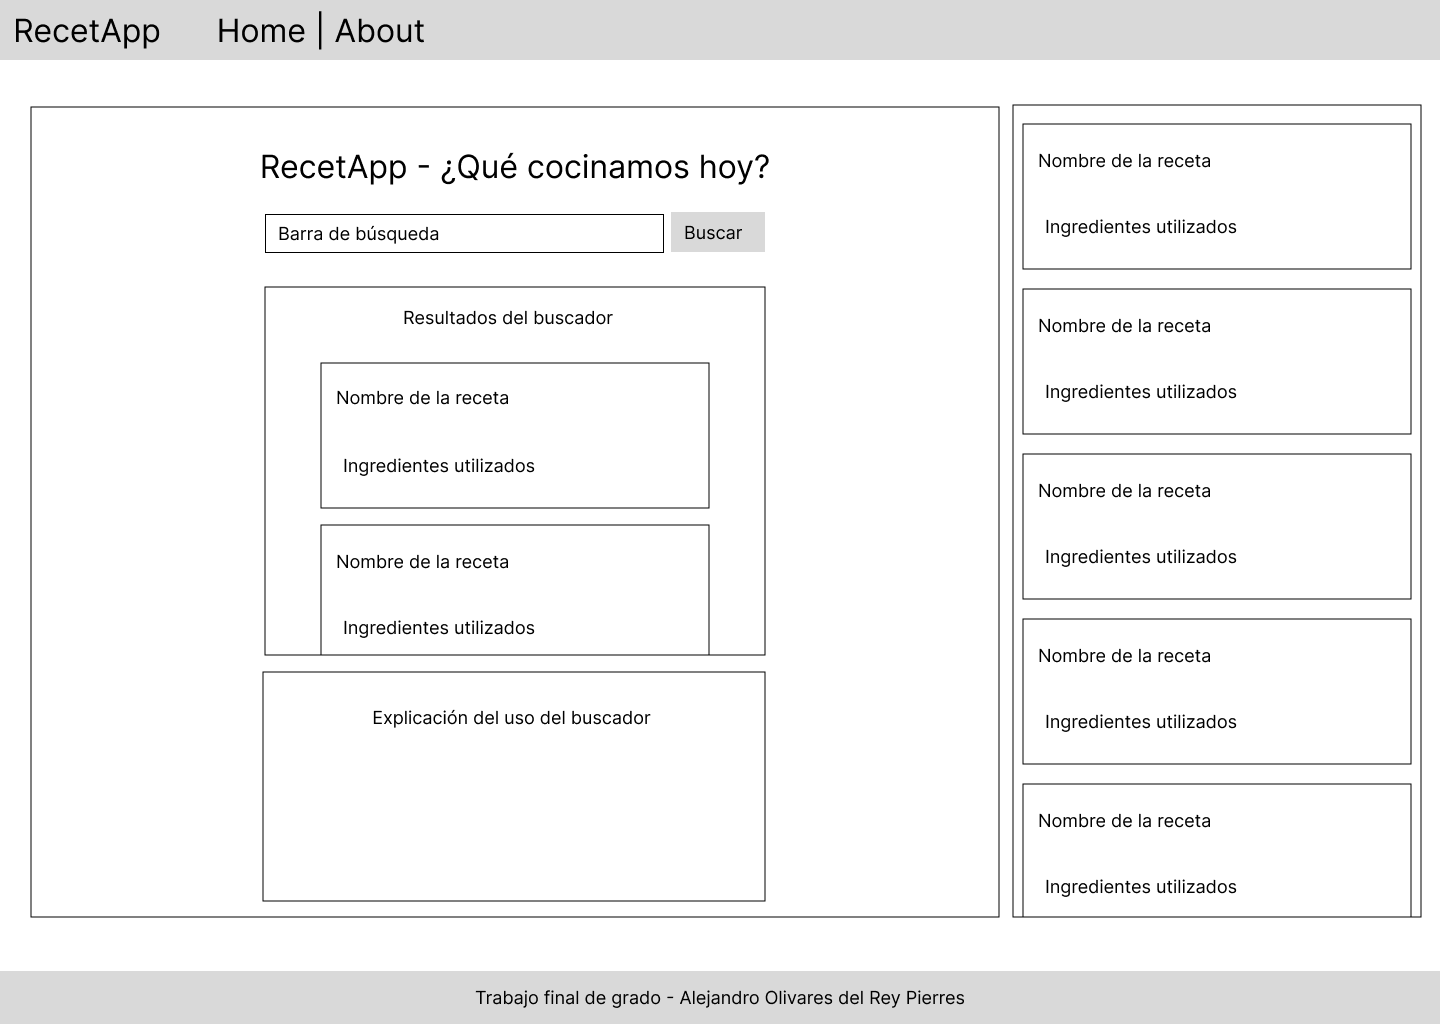
\includegraphics[width=100mm,scale=1]{./doc/imagenes/Desktop.png}}
\caption{Diseño para escritorio}
\label{fig:escritorio}
\end{figure}
En la figura superior se presenta la\gls{interfaz} con un diseño para escritorio. Se utiliza una barra superior a modo de navegador de la página web, con un botón para volver a la página principal y un buscador que permite buscar recetas por nombre. 

En cuanto al diseño central de la aplicación, se puede observar una clara división en dos zonas. El buscador de recetas por ingredientes y una columna a la derecha con algunas recetas aleatorias para inspirar al usuario, estas irán cambiando mientras el usuario utiliza la aplicación. Los resultados del buscador aparecerán bajo la barra de búsqueda.

\subsubsection{Dispositivos móviles}
\begin{figure}[h!]
\centering
\fbox{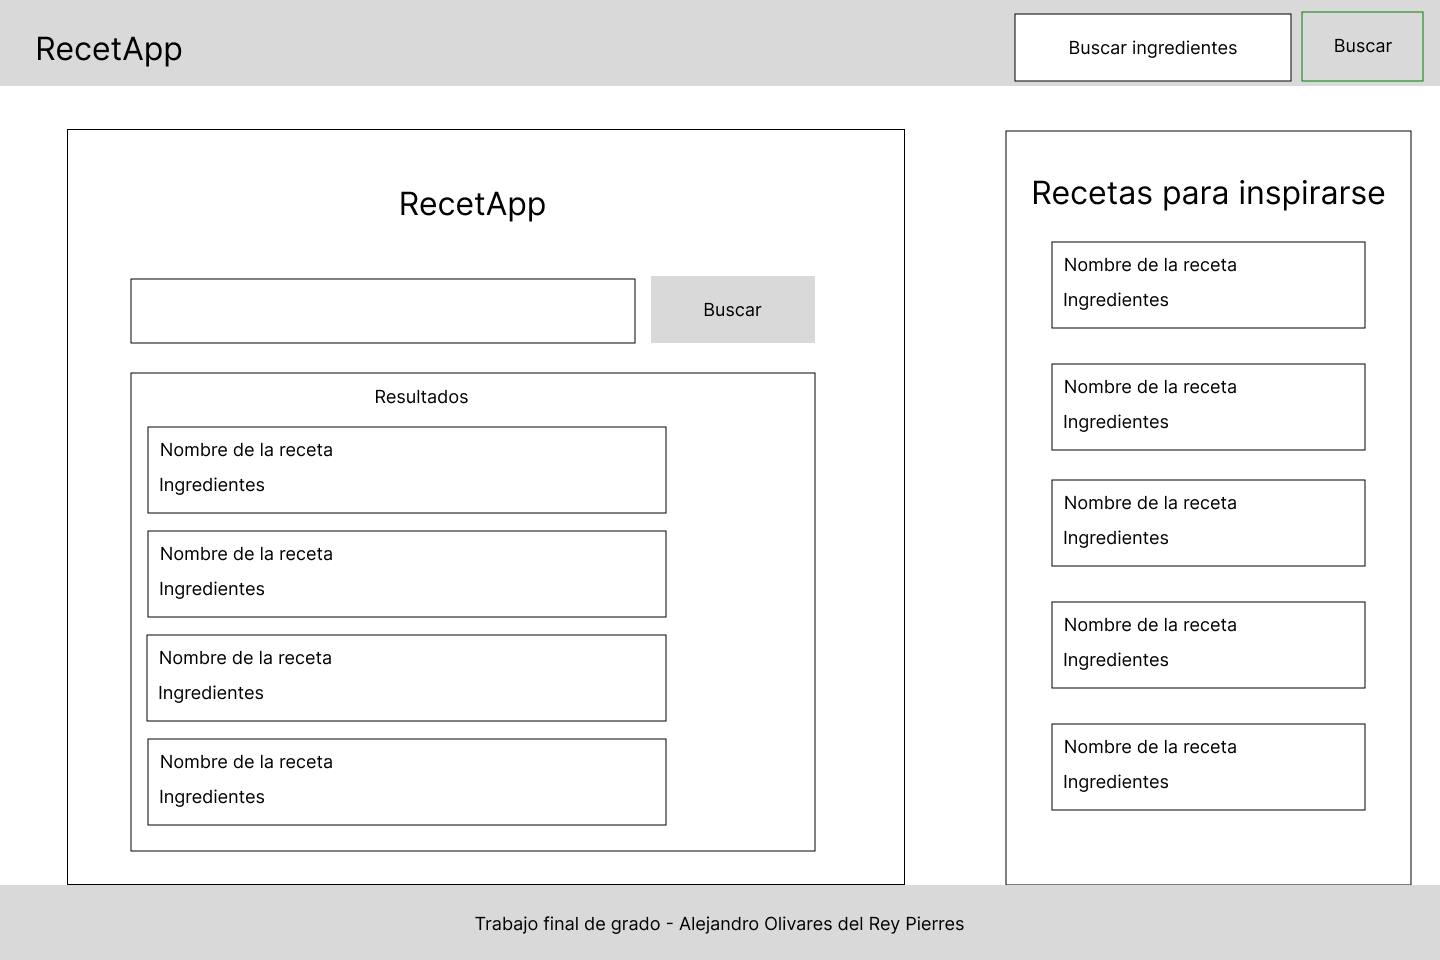
\includegraphics[width=100mm,scale=1]{./doc/imagenes/SurfacePro8.png}}
\caption{Diseño para tableta horizontal}
\label{fig:surface}
\end{figure}
La figura superior muestra un diseño para una tableta en modo horizontal, siendo muy parecida al diseño de escritorio, excepto el navegador que colapsaría mostrando el botón para desplegarlo y la desaparición del cuadro que explicaría el uso del buscador.

\begin{figure}[h!]
\centering
\fbox{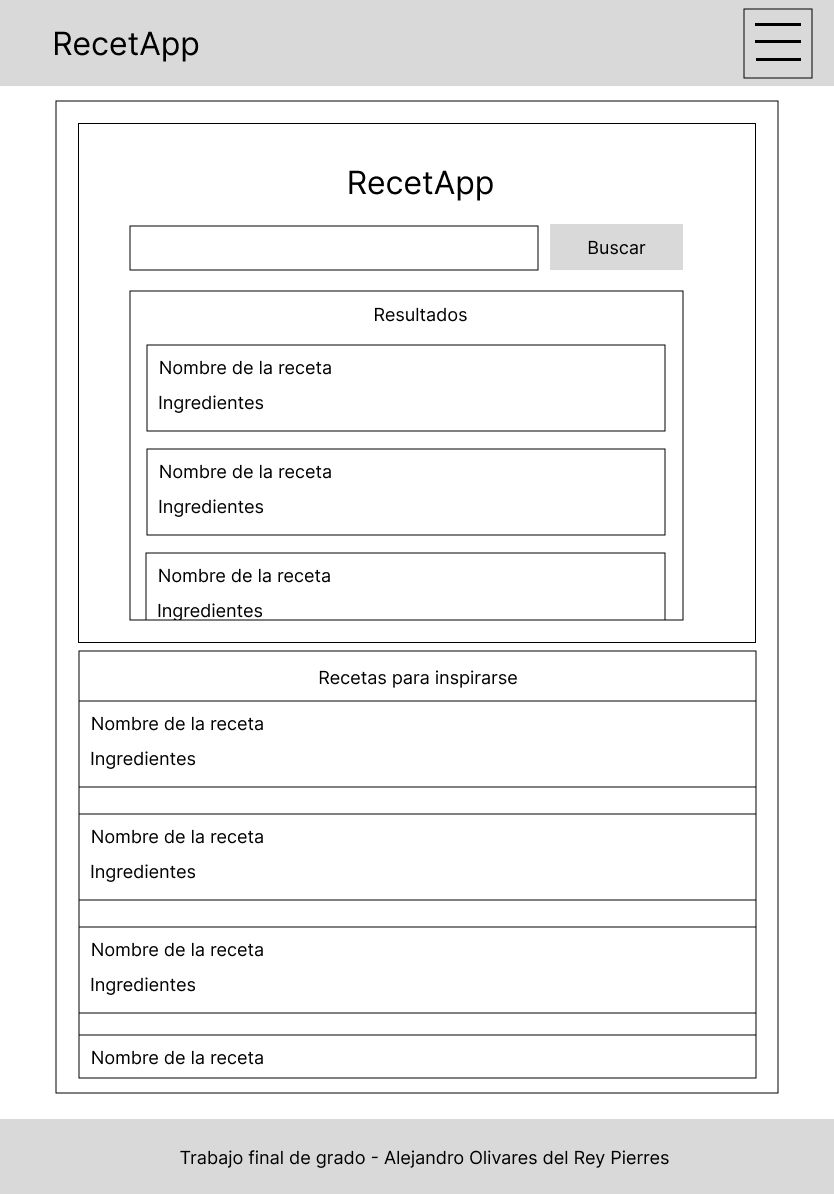
\includegraphics[width=63mm,scale=1]{./doc/imagenes/iPadPro11.png}}
\caption{Diseño para tableta vertical}
\label{fig:ipad}
\end{figure}

\newpage
\section{Uso de git en el proyecto}
\emph{Git} se trata de una herramienta de control de versiones que surge de la necesidad de llevar un seguimiento del código fuente y sus actualizaciones. Es el núcleo de herramientas como \emph{Github} y \emph{Gitlab}. Cualquier equipo de desarrolladores, que cuente con más de un trabajador, debe hacer uso de una de estas herramientas.

Ambas herramientas proporcionan un marco para la gestión de proyectos. Permitiendo que diferentes equipos implementen concurrentemente \emph{features} en el software creando ramas a partir del código principal. Cualquier cambio realizado debe reflejarse con su correspondiente \emph{issue}, dotando de coherencia dichos cambios. Estos no solo sirven para reflejar cambios en el código o correcciones, en un proyecto muy grande también permiten llevar un seguimiento de en que trabaja cada miembro. Todos los \emph{issues} deben estar vinculados a un objetivo o \emph{milestone}. Estos últimos constituyen los entregables (producto mínimo viable) a alcanzar o, lo que es lo mismo, la planificación del proyecto.

Al comenzar todo proyecto, la orientación del mismo se reflejará como una serie de historias de usuario especificadas en \emph{issues} y la planificación haciendo uso de \emph{milestones}.

Para añadir código e ir cerrando \emph{issues}, se utilizan \emph{pull request} (o PR para abreviar). Estas son solicitudes para mezclar código de una rama a otra. Permiten cerrar problemas que pueda tener el código, reflejados en \emph{issues}. Puede darse el caso en el que se quieran mezclar \emph{commits} (o cambios) para cerrar \emph{issues} pero no todos los cambios porque algunos no deben pasar de un \emph{milestone} al siguiente.

En el proyecto ha sido necesario el uso de \emph{cherry-picking} para extraer \emph{commits} de una rama extensa que contenía cambios que no debían mezclarse con la rama principal. Que han sido extraídos a una nueva rama y mezclados con éxito en la rama principal.

\emph{cherry-picking} es un proceso por el cual se escogen \emph{commits} manualmente de una rama para introducirlos en otra. El problema es la dificultad de conocer que cambios contiene cada \emph{commit} y en cual deberían ser introducidos. Se utiliza normalmente en ramas de desarrollo muy largas que no pueden ser mezcladas, los desarrolladores escogen los \emph{commits} haciendo uso de \emph{cherry-pick} y reusar el código en otras ramas.\cite{bunyakiati2017cherry}

Es posible usar \emph{cherry-pick} desde la línea de comandos de git pero es muy lioso, en el proyecto se ha utilizado la herramienta de \href{https://desktop.github.com/}{Github Desktop} para extraer los \emph{commits} de manera sencilla.

\section{Planificación}
En este proyecto se usará una mentalidad ágil para el desarrollo del mismo, esto significa que no se sabe a largo plazo que objetivos se van a cumplir, ya que solo se puede planificar como mucho un objetivo o dos por delante. Pero hasta que no se llega al final de un objetivo no se puede saber realmente por donde se va a seguir avanzando.

Para dar un poco más de contexto, la metodología es la que nos guía para definir el objetivo que debemos alcanzar en cada etapa del proyecto. Una vez que alcanzamos un objetivo, también nos ayuda a establecer el siguiente. En este caso particular, se ha definido únicamente el primer objetivo, que es satisfacer la necesidad del usuario de encontrar recetas. 

Debido a que el desarrollo ágil está centrado en el cliente, no es posible planificar los objetivos que se van a cumplir en el desarrollo del proyecto de antemano.  

En el proyecto se utilizarán \emph{milestones} para medir el desarrollo del progreso, estos son puntos de referencia que indican cuando ha concluido una iteración del desarrollo. También representan un producto mínimo viable o un entregable para el cliente.\cite{milestone2022}

Antes de echarse a definir una solución, el proyecto también requiere de una infraestructura mínima que se debe tener en cuenta para el correcto transcurso del desarrollo ágil. Esta infraestructura constituye como el \href{https://github.com/Slowmybrosh/TFG-DietPlanner/milestone/10}{primer \emph{milestone}} en el proyecto.

Como mínimo, se espera que se elija razonadamente un lenguaje de programación, un gestor de tareas para automatizar llevar a cabo pequeñas labores como la generación de la memoria del proyecto. Por último, se debe añadir un gestor de dependencias que permita fácilmente reproducir el entorno de desarrollo en cualquier computadora que sea necesaria.

El siguiente milestone especificado constituye permitir al usuario encontrar recetas con ciertas restricciones, para ello se establecerán pequeños subobjetivos para alcanzar el milestone y se resolverán cuestiones relativas al objetivo, por ejemplo, que se entiende como ingrediente o receta. Se desestimarán las consideraciones que no avancen el objetivo de cubrir la necesidad del usuario hasta que se complete el milestone relativo a encontrar recetas.

Inicialmente, se especifican los \emph{milestones} mencionados, pero debido a la mentalidad ágil es imposible planificar \emph{milestones} más allá, porque no se sabe que necesidades tendrá el usuario a lo largo del desarrollo del proyecto o que nuevos problemas se pueden plantear y por tanto se especificarán en la sección implementación

\subsection{Milestones}
Para resumir, la lista de \emph{milestones} iniciales mencionados anteriormente son los siguientes\:
\begin{enumerate}
    \item \href{https://github.com/Slowmybrosh/TFG-DietPlanner/milestone/10}{Despliegue de la infraestructura mínima}
    \item \href{https://github.com/Slowmybrosh/TFG-DietPlanner/milestone/3}{Encontrar recetas}
\end{enumerate}